% Overleaf：Menu → Compiler 选 XeLaTeX 或 LuaLaTeX，不要选 pdfLaTeX。
% 本机：在 paper_cscwd2027 目录执行 latexmk main_zh.tex
\documentclass[11pt]{article}

% Chinese setup.
% Overleaf has ctex and the Fandol fonts, but not this machine's Droid font
% or the absolute /data/workspace paths. Use ctex there, and the bundled
% TrueType file only when ctex is absent.
\IfFileExists{ctex.sty}{%
  \usepackage[fontset=fandol]{ctex}%
  \newcommand{\cjkfont}{}%
  \newcommand{\cjkbr}{}%
  \newcount\cjkbreakoff
}{%
  \directlua{tex.enableprimitives("", tex.extraprimitives("pdftex", "luatex"))}%
  \usepackage{fontspec}%
  \defaultfontfeatures{Ligatures=TeX}%
  \IfFileExists{fonts/DroidSansFallback.ttf}{%
    \newfontfamily\cjkfont{DroidSansFallback}[
      Path=fonts/,
      Extension=.ttf,
      UprightFont=*,
      BoldFont=*,
      BoldFeatures={FakeBold=2.4},
      ItalicFont=*,
      ItalicFeatures={FakeSlant=0.16},
      BoldItalicFont=*,
      BoldItalicFeatures={FakeBold=2.4,FakeSlant=0.16}
    ]%
  }{%
    \newfontfamily\cjkfont{DroidSansFallback}[
      Path=../../fonts/,
      Extension=.ttf,
      UprightFont=*,
      BoldFont=*,
      BoldFeatures={FakeBold=2.4},
      ItalicFont=*,
      ItalicFeatures={FakeSlant=0.16},
      BoldItalicFont=*,
      BoldItalicFeatures={FakeBold=2.4,FakeSlant=0.16}
    ]%
  }%
  \DeclareRobustCommand{\cjkbr}{\ifmmode\else\hskip 0pt plus 0.15pt minus 0.05pt\relax\fi}%
  \newcount\cjkbreakoff
  \directlua{%
    local name = "cjkbreak.lua"
    local path = kpse.find_file(name, "tex") or kpse.find_file(name) or name
    dofile(path)
  }%
}

\usepackage{amsmath,amssymb,amsthm}
\usepackage{booktabs}
\usepackage{graphicx}
\usepackage{xcolor}
\usepackage{listings}
\usepackage{enumitem}
\usepackage{cite}
\usepackage{url}
\usepackage[a4paper,margin=1.75cm,headheight=15pt]{geometry}
\usepackage{caption}
\usepackage{indentfirst}
\usepackage{fancyhdr}
\usepackage[unicode,hidelinks]{hyperref}

\setlist[itemize]{leftmargin=1.6em, topsep=3pt, itemsep=2pt, parsep=0pt}
\newlength{\zhindent}
\setlength{\zhindent}{2em}
\newcommand{\parhead}[1]{\par\noindent\hspace*{\zhindent}\textbf{#1}}

\makeatletter
\newtheoremstyle{ieeeitalic}
  {3pt}
  {3pt}
  {\itshape}
  {\zhindent}
  {\bfseries\itshape}
  {：}
  {0pt}
  {\thmname{#1}\thmnumber{~#2}\thmnote{（#3）}}
\theoremstyle{ieeeitalic}
\newtheorem{proposition}{命题}
\renewcommand{\proofname}{证明}

\renewenvironment{proof}[1][\proofname]{\par
  \pushQED{\qed}%
  \normalfont\topsep3pt plus 1pt\relax
  \trivlist
  \item[\hskip\labelsep\hspace*{\zhindent}\bfseries\itshape #1：]\itshape\ignorespaces
}{%
  \popQED\endtrivlist\@endpefalse
}
\makeatother
\renewcommand{\figurename}{图}
\renewcommand{\tablename}{表}
\renewcommand{\refname}{参考文献}

\newcommand{\GS}{\mathrm{GS}}
\newcommand{\dhatmax}{\hat{d}_{\max}}
\newcommand{\Lap}{\mathrm{Lap}}
\newcommand{\RE}{\mathrm{RE}}
\newcommand{\DeriveGS}{\mathsf{DeriveGS}}
\newcommand{\VerifyCert}{\mathsf{VerifyCert}}
\newcommand{\Proj}{\mathsf{Proj}}

\pdfstringdefDisableCommands{\def\cjkbr{}\def\cjkfont{}}

\lstdefinestyle{dslstyle}{
  basicstyle=\ttfamily\small,
  columns=flexible,
  keepspaces=true,
  frame=single,
  rulecolor=\color{black!55},
  framesep=3pt,
  xleftmargin=4pt,
  xrightmargin=4pt,
  aboveskip=6pt,
  belowskip=6pt,
  breaklines=true,
  morekeywords={return,for,in,aggregate,project,size,comb,sum,clip,min,max,pow},
  keywordstyle=\bfseries,
  morecomment=[l]{\#},
  commentstyle=\rmfamily\itshape\color{black!65}
}

\pagestyle{fancy}
\fancyhf{}
\fancyhead[L]{\small CertiCount 中文译文}
\fancyhead[R]{\small 边本地差分隐私下的子结构计数}
\fancyfoot[C]{\thepage}
\renewcommand{\headrulewidth}{0.4pt}

\hypersetup{
  pdftitle={CertiCount：面向边本地差分隐私下子结构计数的验证器引导程序合成与认证执行（中文译文）},
  pdfauthor={Anonymous Authors}
}

\setlength{\parindent}{2em}
\setlength{\parskip}{0.25em}
\setlength{\emergencystretch}{2em}
\tolerance=4000
\hbadness=10000

\begin{document}

\begin{center}
{\LARGE\bfseries CertiCount：面向边本地差分隐私下子结构计数的验证器引导程序合成与认证执行\par}
\vspace{0.7em}
{\large CertiCount: Verifier-Guided Program Synthesis and Certified Execution for Substructure Counting under Local Differential Privacy\par}
\vspace{0.9em}
{\large 匿名作者\par}
\vspace{0.25em}
单位占位\\
Email: placeholder@domain.org
\end{center}

\vspace{0.8em}
\noindent{\large\bfseries 摘要}\par
\vspace{0.3em}
\noindent
大语言模型（LLM）为图分析提供了有前景的自然语言接口，使分析人员无需针对每个查询手工编写专用算法。然而，在敏感的用户连接上计数子结构，必须采用边本地差分隐私（edge-LDP），并且不能把私有边暴露给不可信服务器。若把规则指定和本地计数直接交给多智能体 LLM，会引入若干关键缺陷：节点 LLM 会误计组合模式；把边列表序列化进提示词后，在较大的图上会溢出上下文窗口；把按照理想规则的全局敏感度（$\GS$）校准的噪声加到不稳定的 LLM 输出上，会使差分隐私失效；预设模板或未经验证的策展者规则又限制了安全可扩展性。本文提出 \textbf{CertiCount}，一种验证器引导的程序合成与认证执行框架，在 $\varepsilon$-边 LDP 下把查询设计与私有执行解耦。不可信的策展者 LLM 只访问公开元数据，在确定性检查器诊断所引导的迭代修复下，于受限的图 LDP 领域特定语言（DSL）中合成候选估计器。CertiCount 通过抽象解释静态推导 $\GS$，在合成图上用噪声感知仿真过滤统计退化的估计器，并签发敏感度证书；每个节点在确定性本地执行之前独立重推导该证书，且执行过程不调用节点 LLM。在六个真实数据集上的大量实验表明，CertiCount 在精度和可扩展性上显著优于多智能体 LLM 基线，接近手工设计的专家估计器，并消除了经验上的敏感度违规。此外，诊断修复以更低的 LLM 调用成本明显提高了可发布程序的产出率，并能有效泛化到未见过的子图查询。

\vspace{0.45em}
\noindent\textbf{关键词：}本地差分隐私，图子结构计数，程序合成，敏感度分析，大语言模型

\section{引言}
\label{sec:intro}

计数小型图子结构——例如节点度数、$k$-星、楔形和三角形——是刻画社交、通信、金融和生物网络中连通性、聚类与交互模式的基础\cite{imola2021locally,he2025robust}。随着数据分析日益把大语言模型（LLM）用作自然语言接口\cite{wang2023can,chen2024graphwiz}，分析人员希望提出即席图查询，而不必为每项任务手工设计专用算法。然而，真实网络中的边编码着机密关系，把原始图集中起来会使用户暴露于数据泄露或不可信的策展者\cite{dwork2014algorithmic,imola2021locally}。边本地差分隐私（$\varepsilon$-edge LDP）\cite{imola2021locally,imola2022communication}通过把每个节点的邻居列表留在本地、并在发布前扰动全部出站消息，来降低这一风险。

现有范式面临可扩展性与可信性之间的张力。经典 $\varepsilon$-边 LDP 协议\cite{imola2021locally,imola2022communication,he2025robust,guo2025nam}借助多轮度数界定和偏差校正后的边发布取得较高效用，但要求专家为每种模式推导定制的无偏估计器以及全局敏感度（$\GS$）界，因而难以超出预设模板。与之相对，PSC 等多智能体 LLM 框架\cite{zhang2026psc}通过协调三方来自动化分布式计数：制定计数规则的不可信策展者 LLM、把 $\varepsilon = \varepsilon_1 + \varepsilon_2 + \varepsilon_3$ 拆开的隐私控制器，以及在私有邻居列表上计数本地模式、再加入 $\Lap(\GS/\varepsilon_3)$ 噪声的节点 LLM 智能体。

尽管查询指定被简化了，把 LLM 直接放进规则制定和私有本地执行，会带来三个根本挑战：
\begin{itemize}
    \item \textbf{不可靠的组合执行与上下文瓶颈。}LLM 难以在长上下文上做精确的组合计数\cite{liu2023lost}；把私有邻居列表和稠密的随机响应（RR）含噪边一起序列化成提示词中的节点对文本，会随着图规模增大而溢出上下文窗口\cite{zhang2026psc}，造成严重的计数错误或执行失败。
    \item \textbf{黑盒执行使隐私保证失效。}只有当加噪前的映射敏感度至多为 $\GS$ 时，加入 $\Lap(\GS/\varepsilon_3)$ 噪声才能保证 $\varepsilon_3$-边 LDP\cite{dwork2014algorithmic}。若按理想规则的理论 $\GS$ 来校准噪声，实际却去扰动不稳定的节点 LLM 输出，那么只要一条边的翻转引起不成比例的输出变化，该保证就会被打破。
    \item \textbf{不可信的规则合成与统计退化。}要超出固定模板，就必须在不可信策展者之下合成新的估计器；其提出的逻辑或所声称的 $\GS$ 都可能有误，从而带来静默的隐私违规。此外，即使程序在隐私上有效，如果把非线性组合直接作用到稠密的 RR 扰动行上、又不校正假边，统计上仍会退化。
\end{itemize}

针对这些挑战，本文提出 \textbf{CertiCount}（图~\ref{fig:arch}）。这是一个由严格职责分离所约束的验证器引导合成与认证执行框架：\textbf{LLM 负责设计，系统负责认证，节点执行代码}。LLM 被限制在只针对公开元数据（查询描述与节点数 $n$）的离线循环中；不可信的策展者 LLM 在受限的图 LDP 领域特定语言（DSL）中合成候选估计器。该 DSL 被解析为抽象语法树（AST），并且从不传入 Python \texttt{eval}。在既有边 LDP 原语——逐节点边裁剪\cite{imola2022communication}、无偏含噪邻接矩阵（NAM-DPRD）\cite{guo2025nam}，以及 RR 发布——之上，CertiCount 把策展者 LLM 与确定性的语法、敏感度、语义和小图证伪检查器配对，进行会话内的迭代修复。执行之前，静态分析器（$\DeriveGS$）通过抽象解释推导 $\GS$ 界；在公开合成图上的零预算仿真\cite{holme2002growing,chung2002connected}过滤退化估计器；每个节点再根据公开参数独立重推导并验证敏感度证书（$\VerifyCert$），然后进行确定性本地执行，且不调用节点 LLM。

概括而言，本文有三项主要贡献：
\begin{itemize}
    \item \textbf{解耦的合成与执行架构：}把自然语言查询合成与私有执行解耦，使节点通过确定性解释器运行经认证的 DSL 程序，节点 LLM 调用次数为零，从而在 $\varepsilon$-边 LDP 下消除计数错误和上下文瓶颈。
    \item \textbf{节点可验证的认证与噪声感知选择：}设计受限的图 LDP DSL，具备基于静态抽象解释的 $\GS$ 推导、节点侧独立的证书重推导，以及零预算合成图仿真，用以过滤隐私上有效、但统计上退化的估计器。
    \item \textbf{验证器引导的协作修复与实验验证：}把分阶段的确定性检查器诊断纳入会话内合成，并在六个真实数据集上验证：CertiCount 在效用上接近专家估计器，能防止敏感度违规，以更低的 LLM 成本提高可发布产出率，并能泛化到未见查询。
\end{itemize}

\section{相关工作}
\label{sec:related}

\parhead{边 LDP 下的图子结构计数。}
与集中式图差分隐私\cite{dwork2014algorithmic}不同，$\varepsilon$-边 LDP 在每个用户处本地扰动邻接表。为缓解朴素一轮 RR 图的偏差，Imola 等人\cite{imola2021locally}在全局含噪最大度数下提出了两轮三角形与 $k$-星协议，随后又提出逐节点边裁剪\cite{imola2022communication}，以收紧局部敏感度。后续工作推进了以顶点为中心的三角形估计\cite{he2025robust}、在随机数据上做差分隐私组合的无偏含噪邻接矩阵（NAM-DPRD）\cite{guo2025nam}，以及针对固定模式图的交互协议\cite{chen2026power}。CertiCount 建立在逐节点边裁剪\cite{imola2022communication}和 NAM-DPRD\cite{guo2025nam}之上，而不是引入新的随机化原语，并把这些机制嵌入可验证 DSL，从而自动化估计器合成。

\parhead{用于图分析与多智能体隐私的 LLM。}
已有工作通过图编码、指令微调与多智能体协作，把 LLM 用于图任务\cite{wang2023can,chen2024graphwiz,hu2024scalable}，但 LLM 在精确计数和长边列表上下文上仍然脆弱\cite{liu2023lost}。PSC\cite{zhang2026psc}把 $\varepsilon$-边 LDP 嵌入多智能体 LLM 框架，由节点智能体在拉普拉斯扰动之前计数本地子结构。然而，经验差分隐私审计——借助 Clopper--Pearson 区间\cite{jagielski2020auditing}或 DP-Sniper 等分类器\cite{bichsel2021dpsniper}，在相邻输入上建立隐私损失的下界——表明，放在私有机制内部的黑盒模型可能违反名义敏感度界。CertiCount 把 LLM 完全移出私有执行，并用相邻输入审计\cite{jagielski2020auditing}来说明认证执行的必要性。

\parhead{差分隐私程序验证与验证器引导的合成。}
LightDP\cite{zhang2017lightdp}和 Fuzzi\cite{zhang2019fuzzi}通过关系类型系统与逻辑来验证集中式差分隐私；CheckDP\cite{wang2020checkdp}把证明生成与反例搜索统一起来；DPGen\cite{wang2021dpgen}从无噪声的命令式代码合成噪声机制。与此同时，Self-Refine\cite{madaan2023selfrefine}和 Reflexion\cite{shinn2023reflexion}通过自我批评修改 LLM 输出，但没有可靠性保证；VeriGuard\cite{miculicich2025veriguard}和 DPCheatSheet\cite{chu2025dpcheatsheet}则把 LLM 写代码与静态检查或范例配对。与集中式命令式合成不同，CertiCount 在不可信策展者之下，从自然语言合成去中心化的图 LDP 估计器，并把确定性多阶段修复、由节点重推导的 $\GS$ 证书，以及随机输入上的偏差仿真结合起来。

\section{系统与威胁模型}
\label{sec:model}

\begin{center}
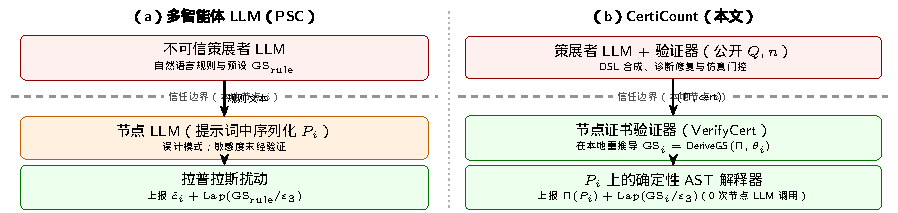
\includegraphics[width=\textwidth]{figures/src/fig1_zh.pdf}
\captionof{figure}{信任边界对比：（a）多智能体 LLM 执行；（b）CertiCount 的认证确定性执行。}
\label{fig:arch}
\end{center}

\parhead{图、查询与信任边界。}
设 $G=(V,E)$ 为无向无权简单图，$n=|V|$，节点为 $\{0,\dots,n-1\}$。每个节点 $i \in V$ 私有地持有其邻接向量 $A_i \in \{0,1\}^n$，即真实邻居集 $P_i = \{j \in V \setminus \{i\} : (i,j) \in E\}$，度数为 $d_i = |P_i|$。给定公开的 $n$、预算 $\varepsilon > 0$ 和自然语言查询 $Q$，系统估计目标计数 $f(G)$。如图~\ref{fig:arch} 所示，策展者与聚合器是\textbf{不可信的}（只能看到公开元数据和扰动后的输出记录，并且可能下发错误程序或被低估的证书）；每个节点 $i$ 运行在\textbf{可信本地服务器}上，$P_i$ 从不进入 LLM 提示词，验证、AST 执行、投影和噪声采样都在本地代码中确定性运行。

\begin{center}
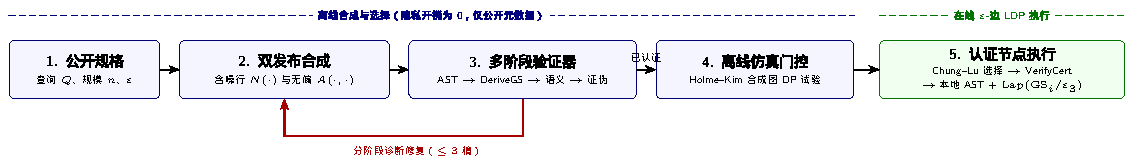
\includegraphics[width=\textwidth]{figures/src/fig2_zh.pdf}
\captionof{figure}{CertiCount 的端到端流水线：先在公开输入上做离线的验证器引导合成与仿真选择（步骤 1--4），再在私有邻居列表上做在线的节点验证执行（步骤 5）。}
\label{fig:pipeline}
\end{center}

\parhead{节点级 $\varepsilon$-边 LDP 与预算划分。}
沿用\cite{imola2021locally,zhang2026psc}，若 $A_i, A_i' \in \{0,1\}^n$ 只在一个比特上不同，则它们相邻（$A_i \sim A_i'$）。若对所有 $A_i \sim A_i'$ 以及可测集 $S$，都有 $\Pr[\mathcal{R}_i(A_i) \in S] \le e^{\varepsilon}\Pr[\mathcal{R}_i(A_i') \in S]$，则节点 $i$ 的联合输出记录 $\mathcal{R}_i(A_i)$ 满足节点级 $\varepsilon$-边 LDP。CertiCount 把 $\varepsilon = \varepsilon_1 + \varepsilon_2 + \varepsilon_3$ 加以划分（未使用的步骤置为 $0$ 并重新缩放）：\footnote{在关系级记账下——一条无向边 $(u,v)$ 会同时改变 $A_u$ 和 $A_v$，而下三角 RR 只扰动 $(u,v)$ 一次——各输出记录上保守的联合预算为 $\varepsilon_1 + 2\varepsilon_2 + 2\varepsilon_3$（第~\ref{sec:discussion}~节）。}
（1）\textbf{度数发布（$\varepsilon_2$）}：节点 $i$ 发布 $y_i = d_i + \Lap(1/\varepsilon_2)$，得到逐节点边裁剪界 $D_i = \lfloor \max(y_i, 0) + \alpha \rfloor$\cite{imola2022communication}（$\alpha \ge 0$），以及全局 $\dhatmax = \min(n-1, \max_j \lfloor \max(y_j, 0) \rfloor)$；
（2）\textbf{边发布（$\varepsilon_1$）}：下三角比特由 Warner 随机响应扰动，翻转概率为 $1/(1+e^{\varepsilon_1})$，形成对称的 $\dhatmax$-投影含噪行 $N(\cdot)$，或者在按 $D_i$ 裁剪后的列表上形成无偏 NAM-DPRD 矩阵\cite{guo2025nam}。其中 $A(j,j)=0$，并且对 $j \neq k$、RR 比特 $\tilde{a}_{jk} \in \{0,1\}$，
\begin{equation}
A(j,k) = \frac{\tilde{a}_{jk}(e^{\varepsilon_1}+1)-1}{e^{\varepsilon_1}-1} \in \Bigl\{-\frac{1}{e^{\varepsilon_1}-1},\, \frac{e^{\varepsilon_1}}{e^{\varepsilon_1}-1}\Bigr\};
\label{eq:nam}
\end{equation}
（3）\textbf{本地计数（$\varepsilon_3$）}：节点 $i$ 上报 $z_i = \Pi(P_i) + \Lap(\GS_i/\varepsilon_3)$，供公开的后处理聚合。在两条显式前提下，由自适应顺序组合\cite{dwork2014algorithmic}可得节点级 $(\varepsilon_1+\varepsilon_2+\varepsilon_3)$-边 LDP：（P1）推导出的 $\GS_i$ 对所有 $P_i \sim P_i'$ 界定 $|\Pi(P_i)-\Pi(P_i')|$；（P2）在一次运行中，节点 $i$ 处的全部 \texttt{project} 调用共享同一个与 $P_i$ 独立的随机顶点顺序。

\section{\texorpdfstring{\textbf{CertiCount} 的设计}{CertiCount 的设计}}
\label{sec:design}

\subsection{系统概览}
\label{sec:overview}

图~\ref{fig:pipeline} 给出了 CertiCount 的工作流。在\textbf{离线合成}（隐私预算为 $0$）中，策展者 LLM 执行两条并行的修复循环——一条面向投影含噪行 $N(\cdot)$，一条面向无偏矩阵 $A(\cdot,\cdot)$（二者都允许只使用私有 $P$ 的程序）——并接收分阶段诊断，最多三稿。经认证的候选在公开的 Holme--Kim 图\cite{holme2002growing}上评估，以丢弃统计退化的估计器并确定预算划分。在\textbf{在线执行}中，若 $N$ 候选与 $A$ 候选在共享的 $\varepsilon_2 > 0$ 下都保留下来，节点先发布 $\{y_i\}$，选择器再在与 $\max(y_i,0)$ 匹配的 Chung--Lu 图\cite{chung2002connected}上挑选误差更低的那一种发布。随后每个节点独立验证证书（$\VerifyCert$），在 $P_i$ 上本地运行 AST，并加入 $\Lap(\GS_i/\varepsilon_3)$ 噪声。

\subsection{图 LDP DSL 与确定性解释器}
\label{sec:dsl}

CertiCount 只通过 \texttt{ast} 解析一个带类型的直线式 Python 子集：以 \texttt{return expr} 结束的单赋值行 \texttt{name = expr}，以及在 \texttt{total}（$\sum_i z_i$）和 \texttt{n} 之上的后处理行 \texttt{aggregate: expr}（结果在 $0$ 处截断）。表达式具有静态类型 \texttt{set}、\texttt{node} 或 \texttt{num}：
\begin{itemize}
    \item \textbf{集合与节点：}\texttt{P}（即 $P_i$，不含 \texttt{self}）、\texttt{N(x)}（投影含噪行）、\texttt{project(S, k)}（至多 $\lfloor k \rfloor$ 个顶点），以及集合运算 \texttt{\&}、\texttt{|}、\texttt{-}；节点为 \texttt{self} 和循环变量。
    \item \textbf{数值与循环：}公开量 \texttt{D}（$D_i$）、\texttt{dmax}（$\dhatmax$）、\texttt{n}；\texttt{A(x, y)}；\texttt{size(S)}；\texttt{comb(x, k)} 与 \texttt{pow(x, k)}（整数常数 $k \ge 0$）；\texttt{clip(x, lo, hi)}；\texttt{min}/\texttt{max}；由非零公开除数进行的 \texttt{+}、\texttt{-}、\texttt{*}、\texttt{/}；以及有界求和 \texttt{sum(e for j in S)}。
\end{itemize}
分支、无界循环、下标、私有除法，以及把 \texttt{N} 与 \texttt{A} 混用，都在解析时被拒绝。下面两段程序分别在含噪行 $N$ 与无偏 NAM-DPRD 矩阵 $A$ 上估计三角形：
{\cjkbreakoff=1
\begin{lstlisting}[style=dslstyle]
# (a) Noisy-row estimator using RR-projected rows N(j)
Q = project(P, D)  # clip private neighbors to bound D_i
return 0.5 * sum(size(Q & N(j)) for j in Q)  # closed wedges
aggregate: total / 3  # 3 vertices report each triangle

# (b) Matrix estimator using unbiased NAM-DPRD entries A(j, k)
Q = project(P, D)  # coupled random-order projection
return sum(sum(A(j, k) for k in Q) for j in Q)  # A(j,j)=0
aggregate: total / 6  # 6 ordered pairs per triangle
\end{lstlisting}
}

\parhead{耦合的随机序投影。}
若多次 \texttt{project} 调用各自抽取独立的随机子集，嵌套表达式上的替换敏感度可能被破坏，例如 $|\texttt{project}(P, D) - \texttt{project}(\texttt{project}(P, 2D), D)|$。为强制前提（P2），耦合算子 $\Proj_\pi$ 在读取 $P_i$ 之前抽取 $V$ 的一个均匀随机置换 $\pi$，并保留 $S$ 在 $\pi$ 下的前 $\lfloor k \rfloor$ 个顶点。因此当 $b \le a$ 时，$\Proj_\pi(\Proj_\pi(S, a), b) = \Proj_\pi(S, b)$；并且 $P_i \sim P_i'$ 对 $\Proj_\pi(P_i, D_i)$ 的改变至多是一次顶点交换（$|\cdot \triangle \cdot| \le 2$，大小变化 $\le 1$）。

\subsection{静态敏感度推导与节点验证}
\label{sec:cert}

给定公开参数 $\theta_i = (n, D_i, \dhatmax, \varepsilon_1)$ 以及图不变量 $\mathcal{F}$（有界对称行，以及非自反的 $P_i$），静态分析器 $\DeriveGS$ 在 AST 上传播抽象界：
\begin{itemize}
    \item \textbf{集合域：}每个集合 $S$ 跟踪 $(\mathrm{priv}, s_{\max}, \Delta_{\mathrm{sym}}, \Delta_{\mathrm{size}})$，用以在 $P_i \sim P_i'$ 下界定 $|S|$、$|S \triangle S'|$ 和 $||S|-|S'||$。\texttt{P} 为 $(\mathrm{true}, n-1, 1, 1)$，\texttt{N(x)} 为 $(\mathrm{false}, \min(\dhatmax, n-1), 0, 0)$，\texttt{project(S, k)} 给出 $(s', \min(2\Delta_{\mathrm{sym}}, 2s'), \min(\Delta_{\mathrm{size}}, s'))$，其中 $s' = \min(s_{\max}, \lfloor k \rfloor)$。把私有集合 $A$ 与公开集合 $B$（$\Delta_{\mathrm{sym}}(B)=0$）相交，可以把大小变化收紧为 $\lfloor (\Delta_{\mathrm{sym}}(A) + \Delta_{\mathrm{size}}(A))/2 \rfloor$，从而把 $|\texttt{project}(P, D) \cap N(j)|$ 的变化界定为 $1$。
    \item \textbf{数值精化：}每个数值跟踪 $(\mathrm{priv}, \delta, [\ell, u], \mathrm{int})$，并使用三条收紧规则：
    （i）\textbf{单变量精确求值}：每当 \texttt{P} 只通过一个整数计数 $X = \texttt{size}(S) \in [\ell, u]$ 进入时，计算 $\max_{|x-y|\le \Delta_X} |g(x)-g(y)|$，从而对 \texttt{comb(size(Q), k)} 和度数多项式都给出 $\binom{D_i-1}{k-1}$；
    （ii）\textbf{替换耦合求和与零对角}：把公开区间 $[\ell, u]$ 上的一次顶点交换界定为 $\max(|\ell|, |u|, u-\ell)$，并丢掉 $A(j,j)=0$，从而对矩阵三角形给出 $2(D_i-1)\bigl(1 + \frac{2}{e^{\varepsilon_1}-1}\bigr)$；
    （iii）\textbf{行对称}以及 $\texttt{self} \notin P_i$，在 \texttt{P \& N(self)} 上给出 $\dhatmax - 1$。
\end{itemize}

\parhead{独立的节点验证。}
给定 $(\Pi, \mathsf{cert})$，其中 $\mathsf{cert} = (\mathrm{digest}(\Pi), \theta_i, \mathcal{F}, \GS_{\mathrm{claim}})$，每个节点运行 $\VerifyCert$：检查 SHA-256 摘要和 $\theta_i$，强制 $\GS_{\mathrm{claim}} \in [0, \infty)$，拒绝其本地强制集合 $\mathcal{F}_{\mathrm{local}}$ 之外的不变量，并重算 $\GS_{\mathrm{own}} = \DeriveGS(\Pi, \theta_i, \mathcal{F}_{\mathrm{local}})$；若 $\GS_{\mathrm{claim}} < \GS_{\mathrm{own}}$ 则中止。

\begin{proposition}[条件性节点级边 LDP]
\label{prop:privacy}
在前提（P1）--（P2）下，对任意策展者输出 $(\Pi, \mathsf{cert})$，仅在 $\VerifyCert$ 成功之后于节点 $i$ 执行 $\Pi$，可使完整的节点输出记录满足 $(\varepsilon_1+\varepsilon_2+\varepsilon_3)$-边 LDP。
\end{proposition}
\begin{proof}[证明概要]
度数发布 $y_i$ 满足 $\varepsilon_2$-LDP（$\GS=1$），$D_i$ 与 $\dhatmax$ 是其后处理；下三角 RR 满足 $\varepsilon_1$-LDP。在以公开输出记录为条件时，$\VerifyCert$ 保证在 $\theta_i, \mathcal{F}_{\mathrm{local}}$ 下有 $\GS_{\mathrm{used}} \ge \GS_{\mathrm{own}}$（是否中止只依赖公开输入）。由（P1）--（P2），$|\Pi(P_i) - \Pi(P_i')| \le \GS_{\mathrm{own}} \le \GS_{\mathrm{used}}$，因此 $\Pi(P_i) + \Lap(\GS_{\mathrm{used}}/\varepsilon_3)$ 满足 $\varepsilon_3$-LDP；再由自适应组合即得结论。
\end{proof}
前提（P1）依赖于人工审计、小图证伪和差分模糊测试（第~\ref{sec:rq2}~节），而不是机械化证明。

\begin{center}
\captionof{table}{六个数据集上 $\varepsilon=2$ 时的平均相对误差 $\RE$（$\downarrow$）。PSC (GPT-4.1) 逐字引自\cite{zhang2026psc}的表~2；PSC (Qwen3)（每格 $10$ 次运行）、GT-PSC（配对运行 $0..99$）和 CertiCount（$20$ 个设计 $\times$ $100$ 次运行）在本文测试床上评估。}
\label{tab:rq1}
\vspace{0.4em}
{\footnotesize
\setlength{\tabcolsep}{5pt}
\renewcommand{\arraystretch}{1.05}
\begin{tabular}{llrrrrrrr}
\toprule
任务 & 方法 & CU & Do & ML & CS & EE & PM & 平均 \\
\midrule
三角形 & GT-PSC & 0.9386 & 0.8655 & 0.4137 & 1.6135 & 0.4012 & 0.9738 & 0.8677 \\
 & PSC (GPT-4.1) & \textbf{0.7939} & 0.8628 & 0.3240 & 2.9922 & 0.2914 & 0.4786 & 0.9571 \\
 & PSC (Qwen3) & 1.1349 & 1.0827 & 0.8857 & 2.4979 & 0.8934 & \multicolumn{1}{c}{---$^\dagger$} & 1.2989$^\dagger$ \\
 & CertiCount & 0.8537 & \textbf{0.6119} & \textbf{0.2296} & \textbf{1.3722} & \textbf{0.2666} & \textbf{0.2744} & \textbf{0.6014} \\
\midrule
度数 & GT-PSC & 0.0216 & 0.0169 & 0.0116 & \textbf{0.0249} & \textbf{0.0057} & \textbf{0.0030} & \textbf{0.0140} \\
 & PSC (GPT-4.1) & \textbf{0.0174} & \textbf{0.0162} & \textbf{0.0110} & 0.0259 & 0.0070 & 0.0666 & 0.0240 \\
 & PSC (Qwen3) & 5.4178 & 23.4054 & 2.5344 & 18.4318 & 30.5186 & 104.1606 & 30.7448 \\
 & CertiCount & 0.0219 & 0.0181 & 0.0130 & 0.0253 & 0.0084 & 0.0055 & 0.0154 \\
\midrule
2-星 & GT-PSC & 0.1408 & 0.0863 & 0.0850 & 0.2002 & 0.0499 & 0.0443 & 0.1011 \\
 & PSC (GPT-4.1) & \textbf{0.0929} & 0.0679 & 0.0563 & \textbf{0.0800} & 0.0349 & 0.3508 & 0.1138 \\
 & PSC (Qwen3) & 0.5816 & 0.4306 & 0.3686 & 0.5081 & 0.4382 & 0.8761 & 0.5339 \\
 & CertiCount & 0.0985 & \textbf{0.0608} & \textbf{0.0388} & 0.1067 & \textbf{0.0250} & \textbf{0.0074} & \textbf{0.0562} \\
\midrule
3-星 & GT-PSC & 0.6632 & 0.3125 & 0.2686 & 0.6120 & 0.1918 & 0.1227 & 0.3618 \\
 & PSC (GPT-4.1) & 0.7325 & 0.3816 & 0.1703 & 0.4711 & 0.2445 & 0.6904 & 0.4484 \\
 & PSC (Qwen3) & 1.1591 & 0.6915 & 0.7404 & 0.8065 & 0.8697 & 1.1177 & 0.8975 \\
 & CertiCount & \textbf{0.4195} & \textbf{0.1783} & \textbf{0.0645} & \textbf{0.2984} & \textbf{0.0402} & \textbf{0.0087} & \textbf{0.1683} \\
\bottomrule
\end{tabular}
\par\vspace{2pt}
{\centering\scriptsize $^\dagger$PSC (Qwen3) 在 PM 的三角形任务上溢出节点提示词上下文；其平均值覆盖 CU--EE（同一范围内 CertiCount 的平均值为 $0.6668$）。\par}
}
\end{center}

\subsection{噪声感知的候选选择与迭代修复}
\label{sec:selection}

只有隐私认证并不足以防止统计退化。例如，\texttt{return comb(size(N(self)), 4)} 的 $\GS=0$，并且能通过无噪声检查（此时 $N(\texttt{self})=P$），但在 RR 假边下会严重高估。此外，有偏的低 $\GS$ 行 $N(\cdot)$ 与无偏、但 $\GS$ 更高的矩阵 $A(\cdot,\cdot)$，在不同密度区间各有优势。CertiCount 采用两种零预算的后处理仿真：
（1）\textbf{设计时门控}：在六张规模为 $n$ 的公开 Holme--Kim 图\cite{holme2002growing}上仿真候选（每张图 $8$ 次试验；度数 $\{4,8,16\}$ 与三元组概率 $\{0.1,0.6\}$ 相乘），丢弃几何平均 $\RE \ge 1.0$ 的任何候选（若一个都不保留，则拒绝发布），并确定预算划分；
（2）\textbf{运行时选择}：若 $N$ 候选与 $A$ 候选共享所选划分且 $\varepsilon_2 > 0$，则在发布 $\{y_i\}$ 之后、执行 $\varepsilon_1$ 与 $\varepsilon_3$ 之前，选择器在三张期望度数为 $\max(y_i, 0)$ 的 Chung--Lu 图\cite{chung2002connected}上对二者做仿真。

\parhead{验证器引导的迭代修复。}
每条合成循环（$\le 3$ 稿）先规范化格式，再按顺序执行六项确定性检查：
（1）\textbf{语法与类型}（带语法提示的 AST 校验）；
（2）\textbf{去重}（规范摘要匹配）；
（3）\textbf{发布与自身行}（强制 $N$ 模式与 $A$ 模式分离，并拒绝含噪的自身查找 \texttt{N(self)} 或 \texttt{A(self,$\cdot$)}，因为节点 $i$ 持有精确的 \texttt{P}）；
（4）\textbf{敏感度紧致性}（拒绝无界 $\GS$，以及在 $D_i, \dhatmax$ 固定时仍随 $4n$ 增长的界）；
（5）\textbf{无噪声语义}（在 $30$ 张无噪声公开图上与暴力计数精确匹配）；
（6）\textbf{小图证伪器}（在 $(n=5, \dhatmax=3)$ 的全部对称图上，以及 $(n=7, \dhatmax=4)$ 的 $500$ 张随机对称图上，对所有投影顺序验证：没有任何一次边翻转会使输出变化超过 $\GS$）。
一旦失败，基础提示保持不变，被拒绝的草稿连同分阶段诊断被附加到一次新的单轮请求中。

\section{实验评估}
\label{sec:eval}

\subsection{实验设置}
\label{sec:setup}

我们评估 PSC\cite{zhang2026psc}中的六个真实网络：Contiguous USA（\texttt{CU}，$n=49$）、Dolphins（\texttt{Do}，$62$）、Les Misérables（\texttt{ML}，$77$）、Ca-sandi\_auths（\texttt{CS}，$86$）、Email-Enron（\texttt{EE}，$143$）以及 \textit{C.~elegans}（\texttt{PM}，$453$）。默认预算为 $\varepsilon=2$\cite{he2025robust,zhang2026psc}，裁剪松弛 $\alpha=5$ 由在 \texttt{CU}/\texttt{Do} 上的预扫描固定。策展者使用 \texttt{Qwen3-8B}（思考模式，温度 $0.6$）。我们把\textbf{设计重复}（每格 $20$ 次合成；RQ3 中为 $30$ 次）与\textbf{噪声重复}（每个被接受的设计运行 $100$ 次；代码基线为 $1{,}000$ 次，并在种子 $0..99$ 上配对）分开，报告相对误差 $\RE = |\hat{f} - f| / \max(f, 0.001n)$\cite{imola2022communication,zhang2026psc}。

在表~\ref{tab:rq1} 中，我们将 CertiCount 与 \textbf{PSC (GPT-4.1)}\cite{zhang2026psc}（GPT-4.1 策展者，GPT-4.1-mini 节点）、骨干匹配的 \textbf{PSC (Qwen3)}（\texttt{Qwen3-8B} 策展者，\texttt{Qwen3-1.7B} 节点，每格 $10$ 次运行）以及 \textbf{GT-PSC}（对 PSC 差分隐私协议的精确 Python 执行）进行比较。对于未见子图查询（表~\ref{tab:rq4}）——\textbf{开放楔}（导出的 $2$-路径）、\textbf{高度数}（满足 $d_i \ge 3$ 的顶点）、\textbf{三角形边}（位于至少 $1$ 个三角形上的边）以及\textbf{三角形节点}（位于至少 $1$ 个三角形上的顶点）——PSC 没有预设规则，因此我们与一轮 RR 计数（\textbf{GT-Naive}）以及在相同裁剪与选择流水线下手工编写的专家 DSL 估计器（\textbf{GT-Expert}）比较。\textbf{三角形}和全部未见查询使用经过泄漏检查的\textbf{零样本语法提示}，其中不含基准范例；单原语的\textbf{度数}与 $k$-星任务则使用较早的\textbf{惯用法增强提示}，其中包含一般性的集合推导重写惯用法。

\subsection{RQ1：效用、可扩展性与节点隐私审计}
\label{sec:rq1}

表~\ref{tab:rq1} 表明，CertiCount 的合成接受率较高（各格为 $80\%$--$100\%$）。相对骨干匹配的 \textbf{PSC (Qwen3)}，平均 $\RE$ 最多降低三个数量级；相对 \textbf{PSC (GPT-4.1)}，在全部四项任务上降低 $1.6\times$--$2.7\times$。关键之处在于，两种范式随图规模 $n$ 的变化方向相反。在 CertiCount 的确定性执行下，各节点独立的拉普拉斯噪声以 $O(\sqrt{n})$ 聚合，而真实计数超线性增长，因此较大网络（\texttt{EE}、\texttt{PM}）上的 $\RE$ 急剧下降\cite{imola2021locally}。相反，多智能体 LLM 执行随着 $n$ 变差，因为更稠密的邻居列表加长了节点提示词：在 \texttt{PM} 的\textbf{度数}任务上，同噪声误差分解表明，差分隐私机制本身只带来 $0.0033$ 的 $\RE$，而节点 LLM 的误计把误差膨胀到超过 $10^2$；在 \texttt{PM} 的\textbf{三角形}任务上，序列化后的邻居列表溢出了节点上下文窗口。

\parhead{经验隐私审计与归因。}
黑盒节点执行还会打破名义上的 LDP 保证。在 \texttt{PM} 的\textbf{度数}任务（$\GS=1, \varepsilon_3=2$）上，我们用 Clopper--Pearson 下界\cite{jagielski2020auditing}（每侧 $300$--$500$ 次新试验，Bonferroni 校正，$\alpha=0.05$）审计 $60$ 个按度数分层的节点。结果确认：\texttt{Qwen3-1.7B} 在 $31/60$ 个节点上、\texttt{Qwen3-8B} 在 $15/60$ 个节点上出现经验 $\varepsilon_3$ 违规（随机下标对照分别为 $7/60$ 和 $4/60$；分层比例并不是全图比率），而 CertiCount 的解释器为 $0/20$。关于机制归因：CertiCount 相对 \textbf{GT-PSC} 的 $k$-星增益，来自用逐节点边裁剪\cite{imola2022communication}替换全局 $\dhatmax$ 投影，从而为低度数节点收紧 $\binom{D_i-1}{k-1}$；在\textbf{度数}（$\GS=1$）上，偶发的度数投影引入轻微截断偏差，使 CertiCount 略低于 \textbf{GT-PSC}。这说明其核心贡献是自动化的认证合成，而不是去超越手工代码。

\subsection{RQ2：认证的可靠性与仿真选择}
\label{sec:rq2}

\begin{center}
\captionof{table}{认证反事实、模糊测试与故障注入。}
\label{tab:rq2}
\vspace{0.35em}
{\footnotesize
\setlength{\tabcolsep}{6pt}
\renewcommand{\arraystretch}{1.08}
\begin{tabular}{lccc}
\toprule
\textbf{评估套件} & \textbf{规模} & \textbf{未认证违规} & \textbf{不健全 / 不安全} \\
\midrule
反事实重放$^\dagger$ & 201 份可运行 & 107（53.2\%，$\ge 28.7\varepsilon_3$） & \textbf{0} \\
端到端合成实验 & 2{,}471 稿 & 752 份可运行违规 & \textbf{0} \\
差分模糊测试（$N$、$A$、节点） & 16{,}000 个程序 & --- & \textbf{0} \\
节点证书故障注入 & 104{,}904 次检查 & --- & \textbf{0}（中位 0.03\,ms） \\
\bottomrule
\end{tabular}
\par\vspace{2pt}
{\raggedright\scriptsize $^\dagger$三角形与开放楔上的全记录子集（共 $302$ 份草稿，其中 $201$ 份在语法上可运行）。\par}
}
\end{center}

表~\ref{tab:rq2} 说明，在不可信策展者之下，静态认证是必要的。若在预设的参考敏感度下重放可运行的 LLM 草稿、而不使用 $\DeriveGS$，则超过一半的可运行草稿会违反名义 $\GS$，最坏情况下的本地隐私损失被放大到 $28\times \varepsilon_3$ 以上。相比之下，在全部 $2{,}471$ 份合成草稿，以及覆盖含噪行、无偏矩阵和逐节点模式的 $16{,}000$ 个差分模糊测试程序中，没有任何一个 $\DeriveGS$ 界被小图证伪所否定；对篡改证书做故障注入（$104{,}904$ 次节点检查）时，不安全接受次数为零，中位延迟为 $0.03$\,ms。同时，用 Holme--Kim 仿真代替无噪声接受，会丢弃受 RR 偏差影响的估计器，从而把 \texttt{PM} 上\textbf{三角形}的 $\RE$ 降低 $6\times$（$1.182 \to 0.197$）。Chung--Lu 运行时选择也能稳定挑出更好的发布：在较大的图上，较低的 $\GS$ 足以抵消 RR 偏差，因而选择 $N(\cdot)$；在较小的聚类图上，则选择无偏的 $A(\cdot,\cdot)$。

\subsection{RQ3：诊断反馈在迭代合成中的作用}
\label{sec:rq3}

\begin{center}
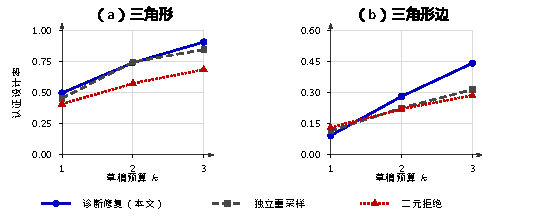
\includegraphics[width=0.92\textwidth]{figures/src/fig3_zh.pdf}
\captionof{figure}{草稿预算 $k \in \{1,2,3\}$ 上的累积认证设计率（每格 $30$ 个设计）。分阶段诊断优于独立重采样和二元拒绝。}
\label{fig:feedback}
\end{center}

为单独考察检查器反馈如何引导合成，我们在相同的初稿提示下，于\textbf{三角形}和\textbf{三角形边}上比较三种变体（每格 $30$ 个设计，每种发布至多 $3$ 稿）：\textbf{诊断修复}（被拒草稿加上分阶段检查器诊断）、\textbf{二元拒绝}（被拒草稿加上仅有的“已拒绝”）以及\textbf{独立重采样}（不携带历史地重试）。图~\ref{fig:feedback} 显示各臂的初稿率一致，说明初始化没有偏置，其后则急剧分化。在全部六个网络上汇总（每臂 $360$ 个设计），\textbf{诊断修复}相对\textbf{独立重采样}把认证发布产出率提高 $+9.2$ 个百分点（Cochran--Mantel--Haenszel 检验 $p = 0.0039$），同时把每个已发布估计器的 LLM 调用减少 $15\%$（在\textbf{三角形边}上为 $28\%$）。相反，\textbf{二元拒绝}比\textbf{诊断修复}低 $18.3$ 个百分点（$p = 1.5\times 10^{-4}$），甚至不如无记忆的重采样：只展示失败草稿、却不指出被违反的不变量，会把 LLM 锚定在近似重复的改写上；而敏感度紧致性诊断和自身行诊断能使下一稿的阶段推进率提高一倍（$73\%$--$86\%$）。

\subsection{RQ4：向未见子图查询的泛化}
\label{sec:rq4}

\begin{center}
\captionof{table}{零样本语法提示下，未见子图查询的平均相对误差 $\RE$（$\downarrow$）（$\varepsilon=2$，每格 $20$ 个设计 $\times$ $100$ 次运行，在种子 $0..99$ 上配对）。}
\label{tab:rq4}
\vspace{0.4em}
{\footnotesize
\setlength{\tabcolsep}{5pt}
\renewcommand{\arraystretch}{1.05}
\begin{tabular}{llrrrrrrr}
\toprule
任务 & 方法 & CU & Do & ML & CS & EE & PM & 平均 \\
\midrule
开放楔 & GT-Naive & 5.1291 & 3.8197 & 3.2747 & 15.3323 & 5.8313 & 9.6771 & 7.1773 \\
 & GT-Expert & \textbf{0.3755} & \textbf{0.2346} & \textbf{0.1590} & \textbf{0.3791} & 0.1812 & 0.0297 & \textbf{0.2265} \\
 & CertiCount & 0.7410 & 0.4184 & 0.3038 & 0.7182 & \textbf{0.1739} & \textbf{0.0292} & 0.3974 \\
\midrule
高度数 & GT-Naive & 0.1370 & 0.3187 & 0.5392 & 1.4566 & 0.1818 & 0.0486 & 0.4470 \\
 & GT-Expert & 0.1077 & 0.1143 & 0.1179 & \textbf{0.1763} & \textbf{0.0585} & \textbf{0.0281} & \textbf{0.1005} \\
 & CertiCount & \textbf{0.1075} & \textbf{0.1139} & \textbf{0.1175} & 0.1766 & 0.0602 & 0.0292 & 0.1008 \\
\midrule
三角形边 & GT-Naive & 0.8628 & 1.5600 & 1.1836 & 4.2415 & 1.8475 & 5.8524 & 2.5913 \\
 & GT-Expert & \textbf{0.4892} & \textbf{0.4833} & 0.4079 & \textbf{0.6340} & \textbf{0.2258} & \textbf{0.1821} & \textbf{0.4037} \\
 & CertiCount & 0.4986 & 0.5648 & \textbf{0.3739} & 0.7128 & 0.2739 & 0.1912 & 0.4359 \\
\midrule
三角形节点 & GT-Naive & \textbf{0.0144} & 0.3354 & 0.3451 & 0.5833 & \textbf{0.1000} & \textbf{0.0203} & 0.2331 \\
 & GT-Expert & 0.2017 & \textbf{0.2203} & 0.2322 & \textbf{0.2411} & 0.1173 & 0.0756 & \textbf{0.1814} \\
 & CertiCount & 0.2167 & 0.2408 & \textbf{0.2085} & 0.2692 & 0.1336 & 0.0743 & 0.1905 \\
\bottomrule
\end{tabular}
}
\end{center}

表~\ref{tab:rq4} 在四项未见子图查询上评估零样本泛化。在\textbf{开放楔}、\textbf{高度数}和\textbf{三角形边}上，CertiCount 在每个数据集上都稳定优于 \textbf{GT-Naive}（总体平均 $\RE$ 降低 $4.4\times$--$18.1\times$），并紧贴手工编写的 \textbf{GT-Expert}；在\textbf{高度数}以及较大网络（\texttt{EE}、\texttt{PM}）上，效用几乎达到专家水平。两种边界情形说明了合成难度与差分隐私噪声结构如何共同起作用：在\textbf{三角形边}上，有界求和内部嵌套的逐邻居指示函数裁剪把合成接受率降到 $35\%$--$55\%$，但被接受的估计器与 \textbf{GT-Expert} 吻合得很紧；在\textbf{三角形节点}上（接受率 $100\%$），CertiCount 在更稀疏的网络（\texttt{Do}、\texttt{ML}、\texttt{CS}）上优于 \textbf{GT-Naive}，并降低了总体平均 $\RE$，但在 \texttt{CU}、\texttt{EE} 和 \texttt{PM} 上落后。在这三张图中，$91\%$--$98\%$ 的顶点位于三角形上，稠密的 RR 图以很小的方差就报告出大约等于 $n$ 的结果。

\section{讨论与局限}
\label{sec:discussion}

\parhead{机械化证明与隐私粒度。}
尽管 $\DeriveGS$ 和 $\VerifyCert$ 在 $2{,}471$ 份草稿与 $16{,}000$ 个模糊测试程序上没有被否定过，前提（P1）仍然缺少机械化定理证明器的验证。沿用\cite{imola2021locally,zhang2026psc}，本文评估采用节点级 $\varepsilon$-边 LDP（$\varepsilon=2$）；若要在两个端点的输出记录上同时保护一条无向边，则需要保守的关系级记账 $\varepsilon_1 + 2\varepsilon_2 + 2\varepsilon_3$（即将 $\varepsilon_2$ 与 $\varepsilon_3$ 减半）。

\parhead{范围、自动化价值与提示的演化。}
实验聚焦于 $\varepsilon=2$ 和 Qwen3 骨干：单原语的\textbf{度数}/$k$-星使用惯用法增强提示，\textbf{三角形}和 RQ4 查询使用零样本语法提示。CertiCount 接近手工编写的 \textbf{GT-Expert}，其价值在于无需为每个查询做专家推导，就能自动化地完成认证合成。按 $O(D_i \dhatmax)$ 增长的高敏感度查询（例如 $4$-环）在 $\varepsilon=2$ 时仍然受边 LDP 噪声的瓶颈制约，并会被仿真门控拒绝。最后，跨任务的提示演化把每次设计的 LLM 调用从 $1.5$--$2.4$ 降到 $1.0$--$1.2$，但没有带来稳定的留出 $\RE$ 改进。这说明，驱动合成可靠性的是会话内的确定性诊断。

\section{结论}
\label{sec:conclusion}

本文提出 CertiCount，在 $\varepsilon$-边 LDP 下把基于 LLM 的估计器合成，与经认证的确定性节点执行解耦。公开元数据上的 DSL 合成、多阶段诊断修复、由节点重推导的敏感度证书，以及零预算仿真选择，共同消除了节点 LLM 的计数错误、上下文溢出失败和经验隐私违规，并能够泛化到未见过的子图查询。

\makeatletter
\let\@mkboth\@gobbletwo
\makeatother
\bibliographystyle{IEEEtran}
\bibliography{references}

\end{document}
